\documentclass[letterpaper,times]{IONconf}
%
% If IONconf.cls has not been installed into the LaTeX system files,
% manually specify the path as follows or keep a copy in the same 
% folder as the document itself:
% \documentclass{../sty/IONconf}

%%%%%%%%%%%%%%%%%%%%%%%%%%%%%%%%%%%%%%%%%%%%%%%%%%%%%%%%%%%%%%%%%%%%%%%%%
% Common packages to import

% ### MATH PACKAGE
\usepackage{amsmath}
\usepackage{amssymb}
\usepackage{bm}
\usepackage{siunitx}

% ### CITATION PACKAGE
%\usepackage{cite}

\usepackage[style=ieee]{biblatex}
\addbibresource{bib.bib}


\usepackage[pdftex]{graphicx}
% to ensure centered multiline captions, the centering package should th
% be called as well.
\usepackage[justification=centering]{caption}
% To use the subfigures command, the subcaption package should be 
% called as well.
\usepackage{subcaption}
\graphicspath{{figs/}}
% To declare their extensions so you won't have to specify these with
% every instance of \includegraphics:
\DeclareGraphicsExtensions{.pdf,.jpeg,.png}


\usepackage{array}
% ### URL PACKAGE
\usepackage{url}

%%%%%%%%%%%%%%%%%%%%%%%%%%%%%%%%%%%%%%%%%%%%%%%%%%%%%%%%%%%%%%%%%%%%%%%%%
%% Document starts here

\title{Bicycle State Estimation with Extended Kalman Filtering of GNSS and Wheel Speed Sensors}

\author{
    Aaron~Wong, \textit{Stanford University}% <- this '%' removes a trailing whitespace
}


\begin{document}
\maketitle

\section{Introduction}

Safe and accurate navigation for cycling in urban environments demands precise localization which the GNSS constellation has the potential to solve. However, single-frequency code phase tracking is only accurate on the order of tens of meters, which is insufficient for accurate localization on streets or lanes.  Code phase GNSS is also susceptible to multipath errors and non-line of sight (NLOS) satellite blocking in dense urban environments which can introduce large errors in position estimates. 

In addition, the receiver is typically assumed to be stationary or subject to simple single integrator dynamics. GNSS only positioning also does not take into account sensors that cyclists typically use to collect dynamic real-time data about their rides, such as power meters, cadence sensors, wheel speed sensors, and cycling computers. 

This report examines using a bicycle specific dynamics model for state prediction. The  nonlinear dynamics are linearized and used as the motion model for an extended Kalman filter that estimates the state of the bicycle. The extended Kalman filter incorporates code phase pseudorange measurements and Doppler shift velocity measurements for state estimation. Also, the wheel speed data from a commercial wheel speed sensor was fused with the GNSS measurements for more precise state estimation. 

This paper is organized as follows. A brief overview of work related to precise urban positioning for cycling is presented. Next, the problem of precise positioning is formally expressed. The details of the dynamics and measurement models used are given and the extended Kalman filter is formulated. Adjustments to the Kalman filter to better tackle facets of this problem are discussed. The results of applying the filter to real-world cycling data are presented and compared to the weighted-least squares pseudorange baseline position solution. Lastly, possible further avenues of investigation are presented.

\section{Related Work}

The problem of precise localization is well studied in the GNSS field, and many augmentation systems have been devised to increase the accuracy of the state estimate. \cite{Witte05} found that the Wide-Angle Augmentation System (WAAS) provides decimeter level precision and accurate velocity estimates, however WAAS-enabled GPS receivers are not typical in consumer level electronics. Also, GNSS augmentation systems usually require the receiver to be in a certain region where corrections are valid, which limits their use around the world. Cyclists will often travel to different countries, but their requirements for precise positioning remain. 

Precise positioning with GNSS is more difficult in urban environments due to urban canyons and limited satellite visibility. Rather than rely only on constellations, high precision localization is typically achieved by The use of external sensors and data fusion with GNSS measurements. For example, both an inertial measurement unit (IMU) and camera in addition to GNSS position estimates are used in \cite{Lategahn13} to estimate position within \SI{10}{cm} in an urban environment. This is very precise, but is designed for  driving applications, where computation power and sensor precision are much higher than expected than on a bicycle. Much of the work of urban positioning seeks to mitigate errors due to signal multipath. \cite{Obst12} uses a 3D environment model to predict and correct multipath in urban areas. As cycling computer have limited memory space, maintaining 3D building models makes these solutions impractical to implement. Multipath and NLOS errors are predicted and corrected for in \cite{Yuan20}, but is only achieved for relative positioning between two receivers. While this has potential for urban navigation, the application to cycling is limited, as cyclists might travel tens of miles from the nearest associated receiver. 

This work aims to provide a cycling specific state estimation filter using typical data collection devices and computation power available to a bicyclist on the road. The problem is detailed in the following section.

\section{Problem Statement}

\newcommand{\R}{R_{ECEF\to ENU}}

For navigation, a cyclist is primarily interested in their position, and velocity. The problem of precise state estimation is to accurately and precisely estimate these values over time given a set of measurements. We will consider measurements to be pseudorange and Doppler shift from GNSS satellites, and wheel speed angular rate from a wheel speed sensor.

For this report, the position of the receiver and the center of mass of the cyclist are assumed to be identical and located at $\vec{p} = [x,y,z]^T$. The velocity of the center of mass is noted as $\vec{v} = [v_x,v_y,v_z]$. Position and velocity can be expressed in the Earth-Centered-Earth-Fixed (ECEF) reference frame $\vec{p}_{ECEF},\vec{v}_{ECEF}$ or the local East-North-Up (ENU) reference frame fixed on the receiver position $\vec{p}_{ENU}(t) = \vec{0},\vec{v}_{ENU}$ which are related by a coordinate transform $\vec{v}_{ENU} [v_E,v_N,v_U]^T = \R{} \vec{v}_{ECEF}$, where $\R$ is a function of the receiver position and thus of time. We assume that the coordinate transform is slowly time varying and its derivative with respect to time is negligible compared to the dynamics of the system. The rotation matrix $\R(p)$ will be abbreviated as $R$ if its meaning is unambiguous. The heading of the vehicle $\theta$ is the angle relative to the local East direction in the East-North plane. The associated in plane speed can be expressed as $v_{EN} = \sqrt{ v_e^2+v_n^2}$. 

Satellite positions and velocities in the ECEF frame $p_{ECEF}^i,v_{ECEF}^i$ are known at the time of transmission from ephemeris data, where $i$ refers to each individual satellite. Satellite clock biases and their rate of change $B^i,\dot{B}^i$ in seconds and seconds per second are also received from ephemeris, and there is assumed to be no error in these values. 

The receiver has some clock bias $b$ and associated clock bias rate $\dot{b}$. For numerical stability, these are expressed in meters and meters per second. The solution setup is described next.

\section{Approach}

\newcommand{\X}{\vec{X}}
\newcommand{\ven}{v_{EN}}


After trying multiple state formulations and dynamics, we settled on the estimated state $\X$ as being 

\begin{align*}
    \X &= [
        \vec{p}_{ECEF}^T , \theta, v_{EN}, b, \dot{b}
    ]^T
\end{align*}

We found that the vertical velocity component $v_U$ was negligible and the evolution of position in the Up direction could be assumed to be due to process noise. This state and its covariance $P$ are passed through an extended Kalman Filter which linearizes the dynamics and measurement models given later. 

For adequate performance of the filter, the filter was then tuned by examining the distributions of innovations and checking that the normalized innovations squared were well described by the $\chi^2$ distribution.

To reduce the effect of NLOS and multipath errors, we attempted to perform elevation masking, Cn0 filtering, innovation testing. However, satellite coverage during data collection was not as good as expected, and elevation masking reduced the number of usable satellites for certain periods. Also, Cn0 values for many visible satellites were not received at each time step, which reduced that viability. Innovation testing proved to reduce some multipath error, but not in some conditions. The details of the nonlinear and linearized dynamics model are given next.

\subsection{Dynamics Model}

Vehicle dynamics are considered in the longitudinal direction, and lateral dynamics are neglected. The vehicle is considered to act under an input force $F $ and steer angle $\psi $. After the driving force, the next most important longitudinal force acting on the bicycle is aerodynamic resistance. Our dynamics model considers the effect of both. The full dynamics model is given in Equation \eqref{eq:dyn}, where $m$ is the cyclist mass, $l$ is the wheelbase of the bike, $rho$ is the density of air, $C_{DA}$ is the aerodynamic coefficient of the cyclist, estimated from \cite{Crouch17}. 

\begin{equation}
    \begin{aligned}
        \dot{\vec{p}}_{ECEF} &= R^T \vec{v}_{ENU} = R^T [\ven \cos \theta , \ven \sin \theta,0]^T\\
        \dot{\theta} &= \frac{ \ven \tan \psi }{l}\\
        \dot{v}_{EN} &= \frac{ 1}{m }( F - \frac{ 1}{2 }\rho C_{DA} \ven^2\mathrm{sign}(\ven))\\
        \dot{b} &= \dot{b}\\
        \ddot{b} &= 0
    \end{aligned} \label{eq:dyn}
\end{equation}

We had previously attempted to include longitudinal slip dynamics in the model, but found that it did not perform well with the linearization required for the extended Kalman filter. In addition, we found that wheel slip averaged only about 4\% over the dataset, which is within the regime where slip dynamics are approximately negligible. 

To linearize the dynamics, the jacobian of the nonlinear dynamics about a set point are calculated in Equation \eqref{eq:jac}. The partial derivatives not calculated are zero for all states. The linearized dynamics are shown in Equation \eqref{eq:lindyn}.

\begin{equation}
    \begin{aligned}
        \frac{ \partial \dot{\X}}{\partial \X } &= 
        \left[ \frac{\partial \dot{\X}} { \partial {\vec{p}}_{ECEF} }, 
        \frac{\partial \dot{\X}} { \partial {\theta} },
        \frac{\partial \dot{\X}} { \partial {\ven} },
        \frac{\partial \dot{\X}} { \partial {b} },
        \frac{\partial \dot{\X}} { \partial {\dot{b}} }
        \right]\\
        \frac{ \partial \dot{\vec{p}}_{ECEF} }{\partial \ven } &= R^T [\cos \theta,\sin \theta, 0]^T\\
        \frac{ \partial \dot{\theta } }{\partial \ven } &= \frac{ \tan \psi }{l }\\
        \frac{ \partial \dot{v}_{EN} }{\partial \ven } &= \mathrm{sign}(\ven) \frac{ \rho C_{DA}}{m } \ven
    \end{aligned} \label{eq:jac}
\end{equation}

\begin{equation}
    \begin{aligned}
        \vec{f}(x_k) &= \vec{X}_{k} + \Delta t \dot{\vec{X}}|_{x_k,u_k=0}\\
        F_k &= \left. \frac{ \partial\vec{f}}{\partial \vec{X}}\right\vert_{\vec{X_{k}}} = I + \Delta t \left.\frac{ \partial \dot{\vec{X}}}{\partial \vec{X} }\right\vert_{\vec{X_k}}
    \end{aligned} \label{eq:lindyn}
\end{equation}


%\begin{align*}
%    \dot{x} &= v_x\\
%    \dot{y} &= v_y\\
%    \dot{\theta } &= V \tan{\psi}\\
%    \dot{v_x} &= \dot{v}\cos{\theta} - v \sin{\theta} \dot{\theta}\\
%    \dot{v_y} &= \dot{v}\sin{\theta} + v\cos{\theta} \dot{\theta}\\
%    \dot{\omega_w} &= \frac{ 1}{I_w }(\tau - \dot{v}mr_w)\\
%    \dot{b_u} &= 0
%\end{align*}

\subsection{Measurement Model}

The wheel speed measurement model is given in Equation \eqref{eq:whl}, where $r_w$ is the radius of the driven wheel. Because the dynamics assume no wheel slip, the wheel speed measurement is assumed to be a linear function of the longitudinal in plane velocity, so the linearized measurement model is accurate within the model.

\begin{equation}
    \begin{aligned}
        \omega &= \frac{ \ven}{r_w } + \epsilon_ \omega  \\
        \frac{ \partial \omega }{\partial \X } &= [0,0,0,0,\frac{ 1}{r_w },0,0]
    \end{aligned} \label{eq:whl}
\end{equation}

The pseudorange measurement model and linearized measurement is given in Equation \eqref{eq:rho}, where $c$ is the speed of light. The simplicity of this linearized equation was part of the motivation of keeping the state position in ECEF but the velocity in ENU frames. 

\newcommand{\norm}[1]{\left\lVert#1\right\rVert}

\begin{equation}
    \begin{aligned}
        \rho^i &= \norm{ \vec{p}^i_{ECEF} - \vec{p}_{ECEF} } + b - cB^i + \epsilon_ \rho \\
        \frac{ \partial \rho^i }{\partial \X } &= \left[\frac{ \vec{p}_{ECEF}^T}{ \norm{ \vec{p}^i_{ECEF} - \vec{p}_{ECEF} } } ,0,0,1,0 \right]
    \end{aligned} \label{eq:rho}
\end{equation}

The Doppler shift or pseudorange rate measurement model and linearized model is described in Equation \eqref{eq:rhor}. $\vec{e}^i$ is the line of sight vector from the receiver to the satellite. Again, all uncalculated partial derivatives are zero.

\newcommand{\prel}{\vec{p}_{rel}}

\begin{equation}
    \begin{aligned}
        \prel &= \vec{p}^i_{ECEF}-\vec{p}_{ECEF}\\
        \vec{e}^i &=  \frac{ \prel }{ \norm{\prel}}\\
        \frac{ \partial \vec{e}^i}{\partial \vec{p}_{ECEF} } &= 
        \frac{ 1}{ \norm{\prel}^{3}} \prel \prel^T - \frac{1}{\norm{\prel}} I_{3\times3}\\
        v_{rel} &= \vec{v}_{ECEF}^i-\vec{v}_{ECEF} = \vec{v}_{ECEF}^i-R^T [\ven \cos \theta, \ven\sin\theta,0]^T\\\\
        \dot\rho &= v_{rel}^T \vec{e}^i + \dot{b} - c\dot{B}^i + \epsilon_{\dot{\rho}}\\
        \frac{ \partial \dot\rho}{\partial \vec{p}_{ECEF} } &= v_{rel}^T \frac{ \partial \vec{e}^i}{\partial \vec{p}_{ECEF} }\\
        \frac{ \partial \dot\rho}{\partial \ven } &= (-R \vec{e}^i)^T [-\ven\sin\theta,\ven\cos\theta,0]^T\\
        \frac{ \partial \dot\rho}{\partial \dot{b} } &= 1
    \end{aligned} \label{eq:rhor}
\end{equation}

Because the wheel speed and GNSS measurements happen asynchronously, they cannot be put into the same measurement model. In addition, the extended Kalman filter needed to be able to handle changing numbers of pseudorange and Doppler shift measurements as satellites enter and leave the view of the receiver. 

One consideration for the GNSS signal is the time of flight calculation, which must be done iteratively by first getting a position estimate to estimate the time of flight. The position is then rotated during the time of flight by the rotation of the Earth, as the satellite transmission point is in inertial space while the receiver is on the surface of the Earth. The estimation of the time of flight is iteratively solved for each satellite at each time step. 

From these models, the extended Kalman filter can be formulated, with the predict and update steps in Equations \eqref{eq:pred} and \eqref{eq:upd}. Note that the time difference $\Delta t$ between $k$ and $k+1$ is variable in this extended Kalman filter.

\begin{equation}
    \begin{aligned}
        \hat{\vec{X}}_{k+1} &= \vec{f}(X_k) \\
        \hat{P}_{k+1} &= F_k P_k F_k^T + Q_k\\
    \end{aligned} \label{eq:pred}
\end{equation}

\begin{equation}
    \begin{aligned}
        \vec{y}_k &= \vec{z}_k - h(\hat{\vec{X}}_k) \\
        S_k &= H_k \hat{P}_{k+1} H_k^T + R_k\\
        K_k &= \hat{P}_{k+1} H_k^T S_k^{-1}\\
        \vec{X}_{k+1} &= \hat{\vec{X}}_{k+1} + K_k \vec{y}\\
        {P}_{k+1} &= (I-K_k H_k)\hat{P}_{k+1}
    \end{aligned} \label{eq:upd}
\end{equation}

The diagonal elements of $P$ correspond to the variance of individual states, and $\vec{y}$ is considered the innovation of the measurement with covariance $S$. The distribution of innovations is the main metric used to tune the filter, described next.

\subsection{Filter Tuning}

\newcommand{\nis}{\mathrm{NIS}}

To tune the covariance matrices of the measurements, we looked at the normalized innovations squared, and the evolution of the state standard deviations compared to the changes in the data. In the Kalman filter, innovations are assumed to be zero mean Gaussian distributed with modelled covariances, because process noise and measurement noise are also Gaussian distributed. The innovations at each time step can be normalized by their covariances $\vec{y}^T S^{-0.5}$ to give an $m$-dimensional that is ideally Gaussian distributed with unit variance. The normalized innovations squared ($\nis$) of a measurement innovation is defined as 

\begin{equation*}
    \nis = \vec{y}^T S^{-1} \vec{y}
\end{equation*}

Which is the sum of squared normalized measurements in each $m$ dimension. This means that the $\nis$ of an innovation is expected to be $\chi^2$ distributed with $m$ degrees of freedom. Examining the $\nis$ over time compared to percentiles of the $\chi^2$ distribution gives a measure of the goodness of fit of a measurement innovation compared to the filter's state prediction. For tuning, we looked at keeping the innovations for pseudorange, Doppler shift, and wheel speed measurements approximately well distributed by the 99\textsuperscript{th} and 65\textsuperscript{th} percentiles of the $\chi^2$ distribution.

For process noise, we examined the time evolution of the state estimates compared to three standard deviation $3 \sigma $ bounds on the state estimates. If the state estimates moved much faster than $3 \sigma $ between each update, this implies that the process noise is not accounting for all noise in the system. But, if the $3 \sigma $ bounds grew faster than the temporal changes in state, the process noise is overestimated and the state estimate could be tighter. 

In addition, some prior knowledge of the dynamics were used to inform process noise estimates. For example, cycling travels much faster horizontally than vertically, so lower process noise was estimated for the vertical direction than East or North.  

The filter also considered the likelihood of each measurement innovation relative to its covariance in an attempt to reduce the effects of multipath. Each innovation was tested against its reported variance. Innovations that deviated significantly from the expectation were removed from the update step.

\section{Results}

The filter was run on an hour of cycling data in the city of Palo Alto. GNSS data was collected from an Android phone that recorded raw code phase GNSS pseudorange and Doppler shift measurements. A Magene wheel speed sensor was used to record wheel speed measurements, and the FIT SDK protocol was used to retrieve the measurements. Position state estimates are compared to the weighted least squares snapshot solution. 

Filter performance is quantitatively judged by the standard deviations of each state estimate, as well as the distribution of $\nis$ for each measurement. Qualitative performance and comparisons are done by examining the position estimate relative to the ground truth map of the roads taken. The resulting EKF solution compared to the weighted least squares snapshots and the ground truth map are shown in Figure \ref{fig:traj}

\begin{figure}
    \centering
    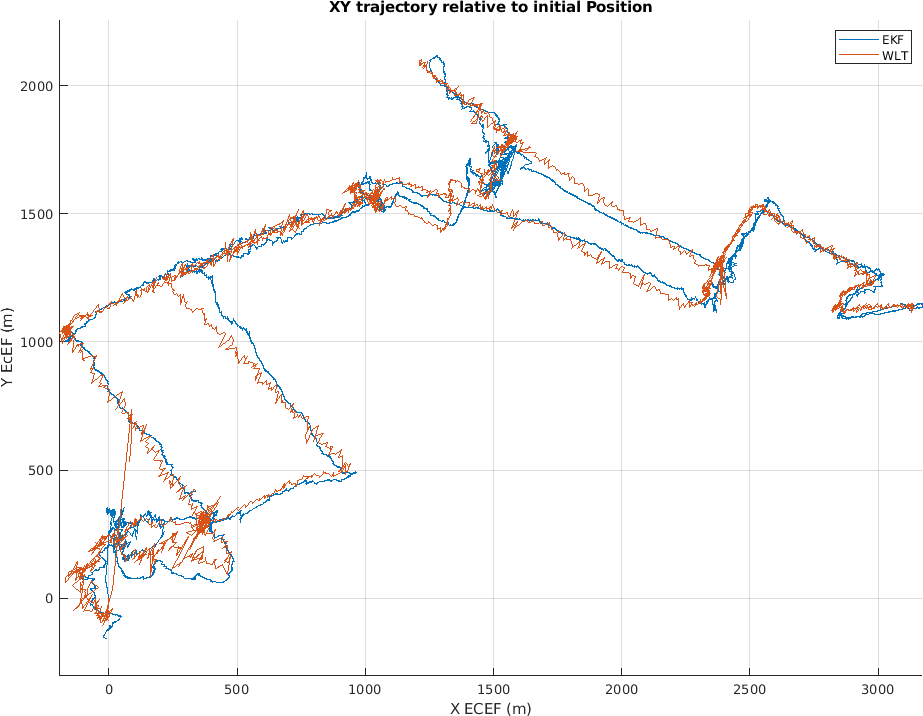
\includegraphics[width=.5\textwidth]{traj}
    \caption{Trajectory of one hour of cycling data. The dataset includes portions of moderately covered residential areas at the beginning and end. The north extent of the data goes by a series of high rises that cause large multipath errors and block satellite visibility.}\label{fig:traj}
\end{figure}

\subsection{Filter Tuning}
The final $\nis$ distribution after tuning is shown in Figure \ref{fig:nis} and $\chi^2$ test consistency comparison are shown in Table \ref{tab:nis}.

\begin{figure}
    \centering
    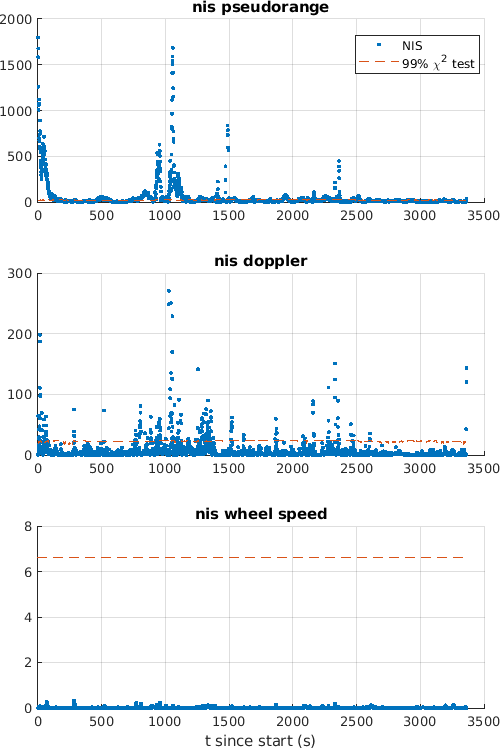
\includegraphics[width=.6\textwidth]{nis}
    \caption{Tuned $\nis$ for each measurement type over time. The initial period of getting the initial fix is clearly shown in the pseudorange and Doppler shift innovations. The high peak around 1000 seconds corresponds to a point of particularly high multipath error, coupled with lower elevation satellites.}\label{fig:nis}
\end{figure}


From the $\nis$ distributions, we can see that the filter is not balanced in weighting each measurement type. Wheel speed measurements should be weighted much higher, but this severely impacted filter estimate performance. In addition, the pseudorange measurements appear to have low consistency, partly due to noticeable regions of the data corrupted by multipath errors.

\begin{table}
    \centering
    \begin{tabular}{l|l|l}
        Measurement & 65\% $\chi^2$ & 99\% $\chi^2$\\
        \hline\hline
        Pseudorange & 44\% & 69\% \\
        Doppler Shift & 87\% & 93\% \\
        Wheel Speed & 100\% & 100\%
    \end{tabular}
    \caption{$\nis$ $\chi^2$ distribution hypothesis tests of each measurement type. Pseudorange measurements are weighted more highly than an ideal filter model, as seen by the percentages being lower than the Chi-squared test percentiles. Likewise, the wheel speed and Doppler shift measurements have higher modelled variance than the data suggests because their percentages are higher than the $\chi^2$ test.}\label{tab:nis}
\end{table}

\subsection{Multipath Filtering}

As an attempt to mitigate the effects of multipath, the update step compares innovations to their standard deviation. Pseudorange and pseudorange rate innovations that are extreme outliers could be due to multipath or NLOS conditions, and are not included when updating the state estimate. A particular example of this is shown in Figure \ref{fig:multi}. 

\begin{figure}
    \centering
    \begin{subfigure}{.45\textwidth}
        \centering
        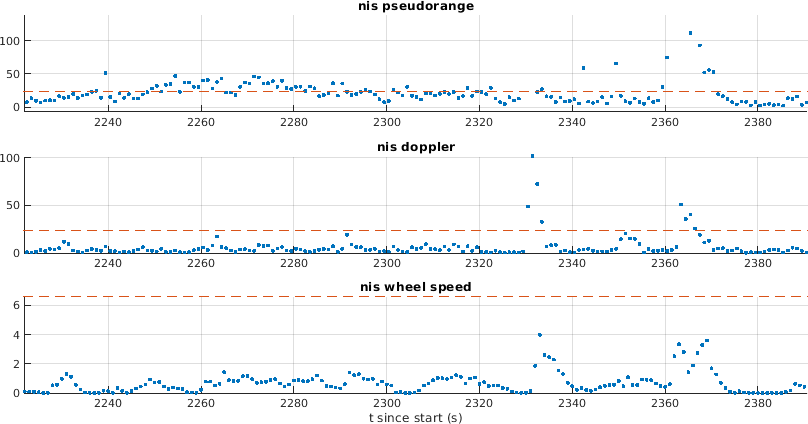
\includegraphics[width=\textwidth]{multi_nis}
        \caption{$\nis$ around the tall Hamilton Apartments to the north of the receiver showing the effects of multipath and satellite blocking.}
    \end{subfigure}
    \begin{subfigure}{.5\textwidth}
        \centering
        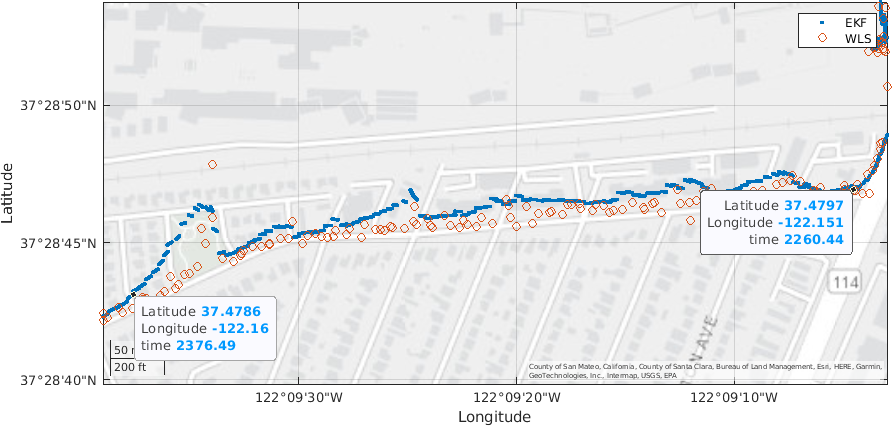
\includegraphics[width=\textwidth]{multi_traj}
        \caption{Unfiltered EKF solution drifts due to multipath errors and a reduced number of satellites in view.}
    \end{subfigure}
    \begin{subfigure}{.5\textwidth}
        \centering
        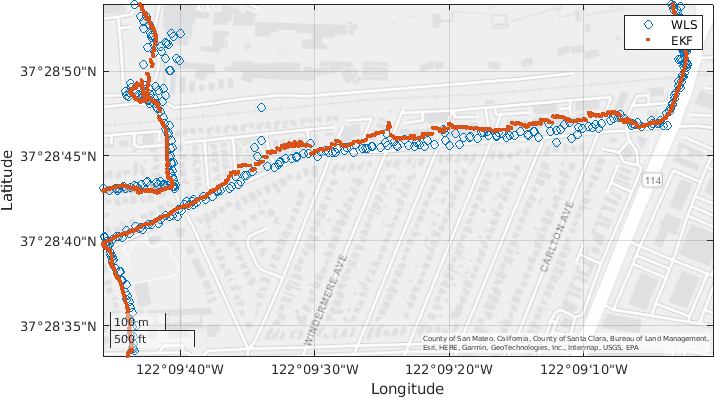
\includegraphics[width=\textwidth]{multi_filter}
        \caption{Filtered EKF solution rejects some bias due to multipath and maintains a better estimate of the state.}
    \end{subfigure}
    \caption{Example of multipath and its effect on state estimation, as well as the filter's attempt to reduce the effects of multipath.} \label{fig:multi}
\end{figure}

The filter does a particularly good job of filtering out errant pseudorange measurements when the receiver is stationary, shown in Figure \ref{fig:stationary}.

\begin{figure}
    \centering
    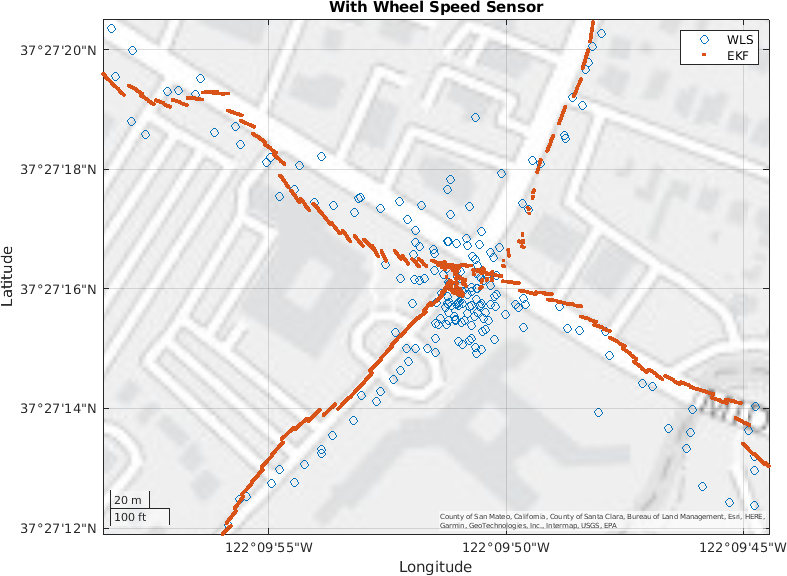
\includegraphics[width=.7\textwidth]{intersect_whl}
    \caption{Due to the informed motion model for the EKF, the position fix when receiver velocity is low is much better than the weighted least squares solution. In these situations, the EKF successfully filters out pseudorange noise that is in the snapshot solutions.}\label{fig:stationary}
\end{figure}

\subsection{State Estimation}

The resulting state standard deviations are shown in Figure \ref{fig:std}, and a summary of the distribution of standard deviations is given in Table \ref{tab:std}. These deviations are tight enough to localize the cyclist to a one or two lanes on a typical road, which is suitable enough for bike-lane specific navigation in an urban environment. We expect that part of the positional variance is due to the relatively high variance of the heading of the vehicle, which is where most of the nonlinearity of the system lies. With higher quality sensors or an additional sensing mode, the state estimate could be even tighter. 

\begin{figure}
    \centering
    \begin{subfigure}{.47\textwidth}
        \centering
    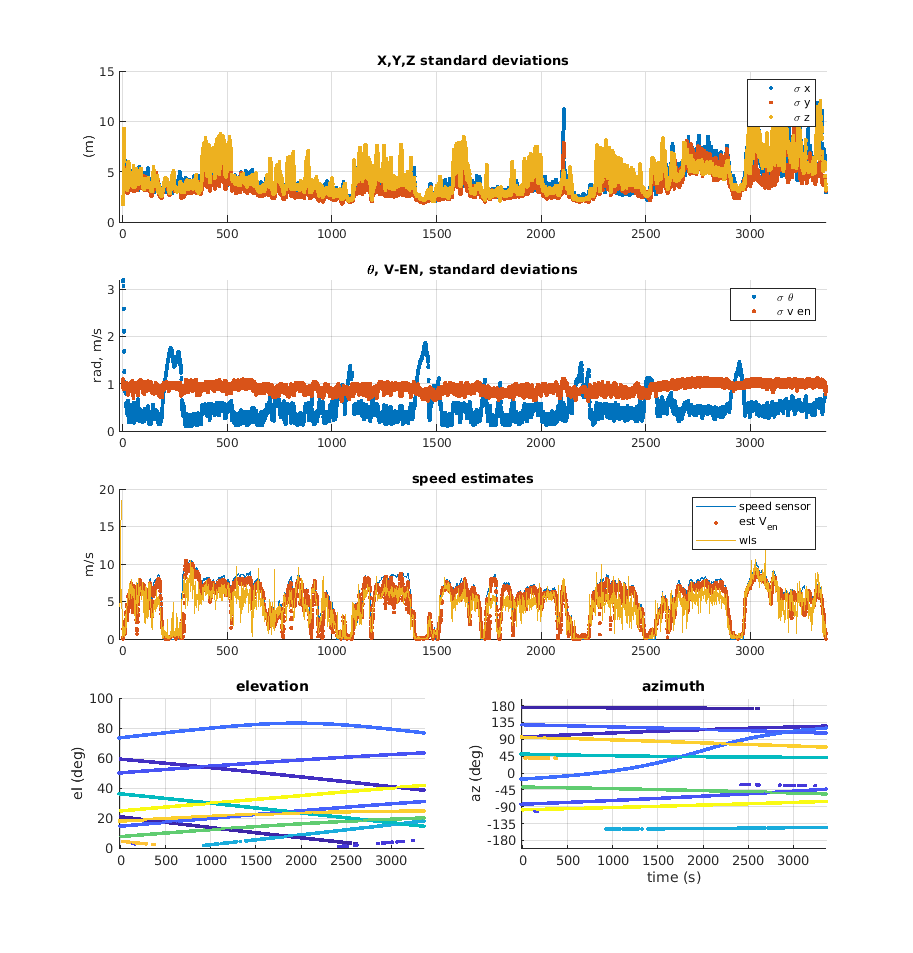
\includegraphics[width=\textwidth]{std_devs}
    \caption{Standard deviations in position, velocity, and heading over time. The speed estimate is compared to that of  the weighted least squares solution and the prediction of the wheel speed sensor. Elevation and azimuth of all satellites are also shown. Note that only a handful of low elevation satellites give visibility from the South, which contributes to the  large effects of multipath.}
        \end{subfigure}
        \begin{subfigure}{.47\textwidth}
    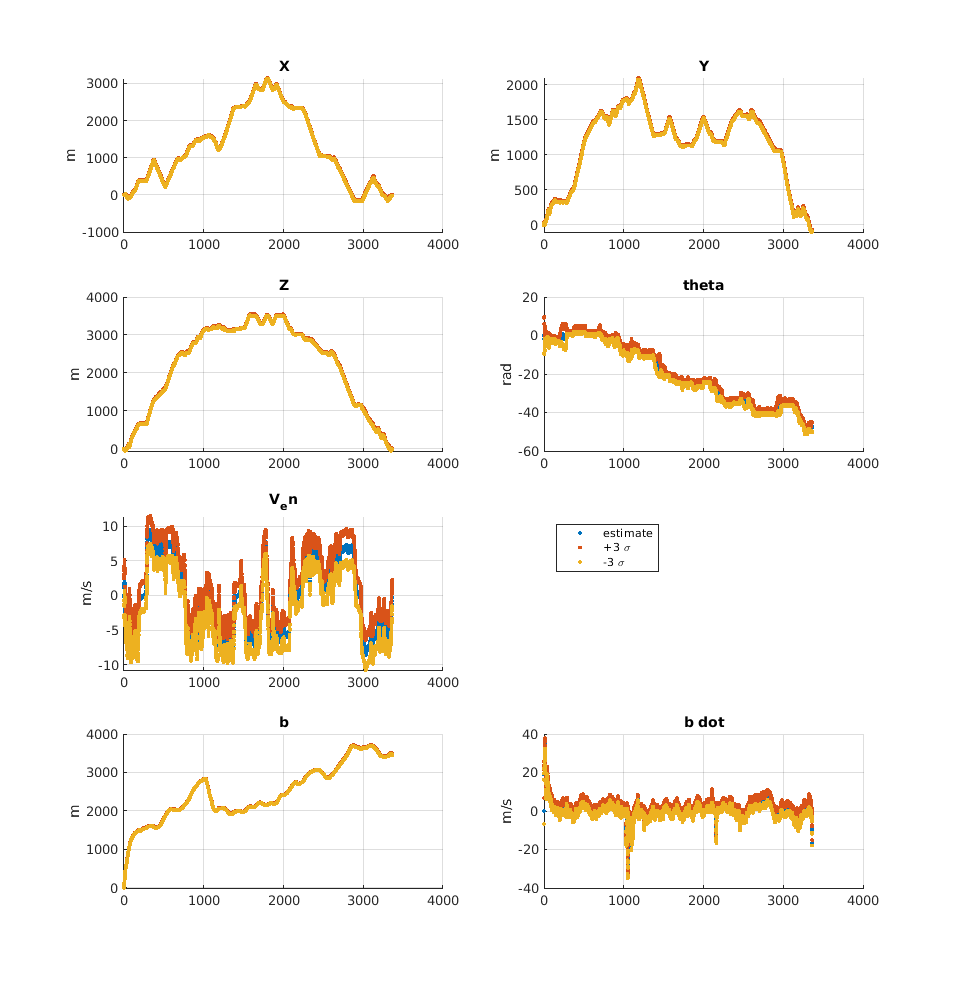
\includegraphics[width=\textwidth]{3_sigs}
            \caption{Three-$\sigma$ bounds on the estimated states. Position states are approximately bound by $\pm\SI{5}{\m}$, $\theta$ by $\pm\SI{1}{\radian}$, and velocity by $\pm \SI{2}{\m\per\s}$ }
    \end{subfigure}
    \caption{Standard deviation and three-$\sigma $ bounds on states over time.} \label{fig:std}
\end{figure}

\begin{table}
    \centering
    \begin{tabular}{l|l|l}
        State & 50\% $\sigma$ & 95\% $\sigma$\\
        \hline\hline
        x & 3.59 m & 6.70 m\\
        y & 3.28 m & 5.77 m\\
        z & 3.99 m & 7.44 m\\
        $\theta$ & \SI{0.47}{\radian} & \SI{1.18}{\radian}\\
        $\ven$ & 0.64 m/s & 0.75 m/s\\
    \end{tabular}
    \caption{Standard deviations of navigation states, 50\textsuperscript{th} and 95\textsuperscript{th} percentiles.}\label{tab:std}
\end{table}

\section{Conclusions and Future Directions}

Filter performance with wheel speed measurements was unfortunately only  marginally better than the EKF solution with only GNSS measurements. A major limitation to the wheel speed sensor was that it only output data at \SI{1}{\hertz} which was not high enough to perform wheel odometry. In addition, the sensor might not have been calibrated to accurately measure the wheel speed and might perform lower level filtering or averaging of the output per reading. There might also have been some issues synching the timestamps of the GNSS measurements and wheel speed measurements.

Overall, EKF sensor fusion applied to a bicycle specific motion model shows promise for giving precise positioning in urban environments. The EKF provided lane-accurate positioning through carrier-phase GNSS and wheel speed measurements. Further work could explore using a higher refresh rate wheel speed sensor or code-phase GNSS for more precise position estimation. IMU sensors on either the cyclist or fixed to the vehicle could be used for higher derivative state estimation. Also, a power meter or camera unit attached to the handlebars could be used to generate control input signals that would reduce the process noise of the system greatly. 


% the IEEE bibliography style matches the ION bibliography style guidelines.
%\bibliographystyle{IEEEtran}
\printbibliography{}

\end{document}
